
%%%%%%%%%%%%%%%%%%%%%%%%%%%%%%%%%%%%%%%%%%%%%%%%%%%%%%%%%%%%%%%%%%%%%%%%%%%%%%%
\section{Hydrodynamics Test Problems}

\subsection{Sod's Problem (and Other Shock Tube Problems)}

The {\tt Exec/hydro\_tests/Sod} problem directory sets up a general one-dimensional
shock tube.  The left and right primitive-variable states are specified
and the solution evolves until a user-specified end time.  For a simple
discontinuity, the exact solution can be found from an exact Riemann 
solver.  For this problem, the exact solutions were computed with the
exact Riemann solver from Toro \cite{toro:1997}, Chapter 4.

\subsubsection{Sod's Problem}

The \problem{Sod} problem \cite{sod:1978} is a simple shock tube problem that
exhibits a shock, contact discontinuity, and a rarefaction wave.
The initial conditions are:
\begin{equation}
\begin{array}{l}
\rho_L = 1 \\
u_L = 0 \\
p_L = 1
\end{array}
\qquad
\begin{array}{l}
\rho_R = 0.125 \\
u_R = 0 \\
p_R = 0.1
\end{array}
\end{equation}
The {\tt gamma\_law} equation of state is used with $\gamma = 1.4$.
The system is evolved until $t = 0.2$~s.  Setups for 1-, 2-, and 3-d
are provided.  The following inputs files and probin files setup the
Sod's problem:
\begin{table*}[h]
\centering
\begin{tabular}{|l|l|l|} \hline
\multicolumn{1}{|c}{\em inputs file} &  \multicolumn{1}{|c}{\em probin file} & \multicolumn{1}{|c|}{\em description} \\
\hline
{\tt inputs-sod-x} & {\tt probin-sod-x} & Sod's problem along $x$-direction \\
{\tt inputs-sod-y} & {\tt probin-sod-y} & Sod's problem along $y$-direction \\
{\tt inputs-sod-z} & {\tt probin-sod-z} & Sod's problem along $z$-direction \\
\hline
\end{tabular}
\label{Table:Sod}
\end{table*}

For multi-dimensional runs, the directions transverse to the jump are
kept constant.  We use a CFL number of 0.9, an initial timestep shrink
({\tt castro.init\_shrink}) of 0.1, and the maximum factor by which
the timestep can increase ({\tt castro.change\_max}) of 1.05.
\begin{figure}[h]
\centering
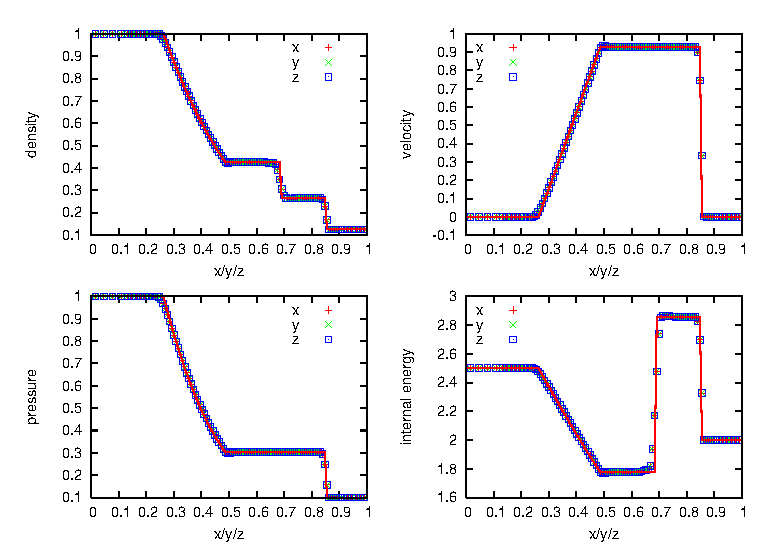
\includegraphics[width=4.75in]{sod_3d}
\caption{\label{fig:sod} \castro\ solution for Sod's problem run in 3-d,
  with the newest ppm limiters, 
  along the $x$, $y$, and $z$ axes.  A coarse grid of 32 zones in the
  direction of propagation, with 2 levels of refinement was used.  The
  analytic solution appears as the red line.}
\end{figure}
\begin{figure}[h]
\centering
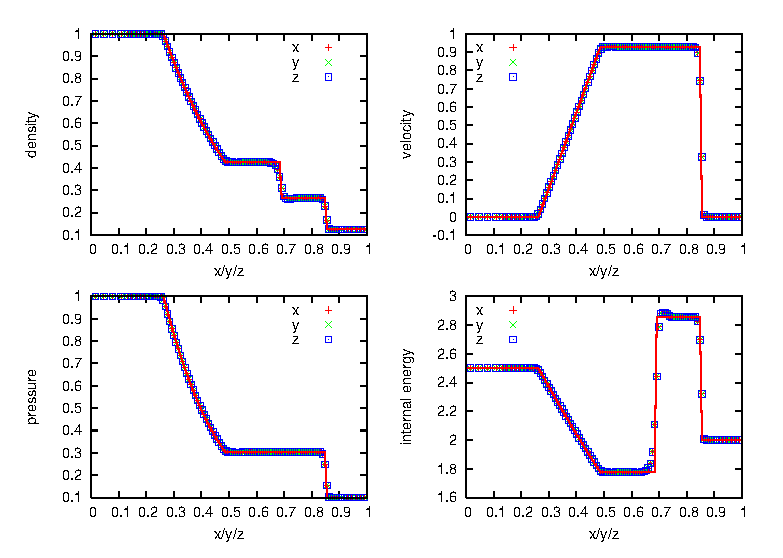
\includegraphics[width=4.75in]{sod_3d_ppm0}
\caption{\label{fig:sod_ppm0} \castro\ solution for Sod's problem run in 3-d,
  with the piecewise-linear Godunov method with limiters,
  along the $x$, $y$, and $z$ axes.  A coarse grid of 32 zones in the
  direction of propagation, with 2 levels of refinement was used.  The
  analytic solution appears as the red line.}
\end{figure}

Figure~\ref{fig:sod} shows the \castro\ solution using the newest PPM limiters
compared to the analytic 
solution, showing the density, velocity, pressure, and internal energy.
Figure~\ref{fig:sod_ppm0} is the same as Figure~\ref{fig:sod},
but with the piecewise-linear Godunov method with limiters, 
shown for comparison.

The {\tt Verification} subdirectory includes the analytic solution for
the Sod problem {\tt sod-exact.out}, with $\gamma = 1.4$.  1-d slices
can be extracted from the \castro\ plotfile using the {\tt fextract} tool
from {\tt BoxLib/Tools/Postprocessing/F\_Src/}.  
The steps to generate this verification plot with \castro\ are:
\begin{enumerate}
\item in {\tt Exec/hydro\_tests/Sod}, build the \castro\ executable in 3-d
\item run the Sod problem with \castro\ in the $x$, $y$, and $z$ directions: \\
 {\tt ./Castro3d.Linux.Intel.Intel.ex inputs-sod-x} \\
 {\tt ./Castro3d.Linux.Intel.Intel.ex inputs-sod-y} \\
 {\tt ./Castro3d.Linux.Intel.Intel.ex inputs-sod-z}
\item build the {\tt fextract} tool in {\tt BoxLib/Tools/Postprocessing/F\_Src/}.  
\item run {\tt fextract} on the \castro\ output to generate 1-d slices
 through the output: \\
 {\tt fextract3d.Linux.Intel.exe -d 1 -s sodx.out -p sod\_x\_plt00034} \\
 {\tt fextract3d.Linux.Intel.exe -d 2 -s sody.out -p sod\_y\_plt00034} \\
 {\tt fextract3d.Linux.Intel.exe -d 3 -s sodz.out -p sod\_z\_plt00034}
\item copy the {\tt sodx/y/z.out} files into the {\tt Verification} directory.
\item in {\tt Verification} run the gnuplot script {\tt sod\_3d.gp} as: \\
 {\tt gnuplot sod\_3d.gp} \\
 This will produce the figure {\tt sod\_3d.eps}.
\end{enumerate}

\subsubsection{Double Rarefaction}

The double rarefaction is the ``Test 2'' problem described by Toro
\cite{toro:1997}, Chapter 6.  In this test, the center of the domain
is evacuated as two rarefaction waves propagate in each direction, outward
from the center.  It is difficult to get the internal energy to 
behave at the center of the domain because we are creating a vacuum.
The initial conditions are:
\begin{equation}
\begin{array}{l}
\rho_L = 1 \\
u_L = -2 \\
p_L = 0.4
\end{array}
\qquad
\begin{array}{l}
\rho_R = 1 \\
u_R = 2 \\
p_R = 0.4
\end{array}
\end{equation}
The {\tt gamma\_law} equation of state is used with $\gamma = 1.4$.
The system is evolved until $t = 0.15$~s.  Setups for 1-, 2-, and 3-d
are provided.  The following inputs files and probin files setup the
Sod's problem:
\begin{table*}[h]
\centering
\begin{tabular}{|l|l|l|} \hline
\multicolumn{1}{|c}{\em inputs file} &  \multicolumn{1}{|c}{\em probin file} & \multicolumn{1}{|c|}{\em description} \\
\hline
{\tt inputs-test2-x} & {\tt probin-test2-x} & Double rarefaction problem along $x$-direction \\
{\tt inputs-test2-y} & {\tt probin-test2-y} & Double rarefaction problem along $y$-direction \\
{\tt inputs-test2-z} & {\tt probin-test2-z} & Double rarefaction problem along $z$-direction \\
\hline
\end{tabular}
\label{Table:Sod}
\end{table*}

We use a CFL number of 0.8, an initial
timestep shrink ({\tt castro.init\_shrink}) of 0.1, and the maximum factor by which
the timestep can increase ({\tt castro.change\_max}) of 1.05.  The PPM
solver with the new limiters are used.
\begin{figure}[h]
\centering
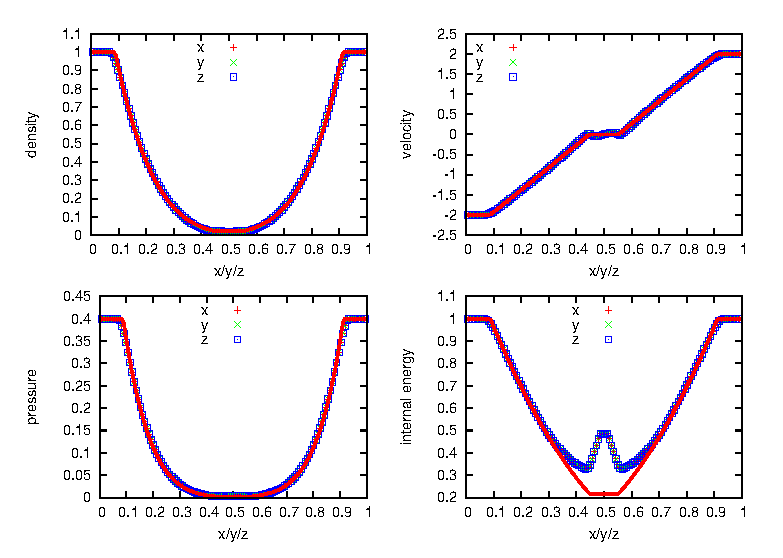
\includegraphics[width=5.0in]{test2_3d}
\caption{\label{fig:test2} \castro\ solution for the double rarefaction
  problem run in 3-d, along the $x$, $y$, and $z$ axes.  A coarse grid
  of 32 zones in the direction of propagation, with 2 levels of
  refinement was used.  The analytic solution appears as the red
  line.}
\end{figure}

Figure~\ref{fig:test2} shows the \castro\ output, run along all 3
coordinate axes in 3-d, compared to the analytic solution.  

The comparison to the analytic solution follows the same procedure as
described for the Sod's problem above.  The gnuplot script {\tt
  test2\_3d.gp} will generate the figure, from the 1-d slices created by
{\tt fextract} named {\tt test2x.out}, {\tt test2y.out}, and {\tt test2z.out}.

\subsubsection{Strong Shock}

The strong shock test is the ``Test 3'' problem described by Toro
\cite{toro:1997}, Chapter 6.  In this test, a large pressure jump
at the initial interface creates a very strong rightward moving
shock, followed very closely by a contact discontinuity.
The initial conditions are:
\begin{equation}
\begin{array}{l}
\rho_L = 1 \\
u_L = 0 \\
p_L = 1000
\end{array}
\qquad
\begin{array}{l}
\rho_R = 1 \\
u_R = 0 \\
p_R = 0.01
\end{array}
\end{equation}
The {\tt gamma\_law} equation of state is used with $\gamma = 1.4$.
The system is evolved until $t = 0.012$~s.  Setups for 1-, 2-, and 3-d
are provided.  The following inputs files and probin files setup the
Sod's problem:
\begin{table*}[h]
\centering
\begin{tabular}{|l|l|l|} \hline
\multicolumn{1}{|c}{\em inputs file} &  \multicolumn{1}{|c}{\em probin file} & \multicolumn{1}{|c|}{\em description} \\
\hline
{\tt inputs-test3-x} & {\tt probin-test3-x} & Strong shock problem along $x$-direction \\
{\tt inputs-test3-y} & {\tt probin-test3-y} & Strong shock problem along $y$-direction \\
{\tt inputs-test3-z} & {\tt probin-test3-z} & Strong shock problem along $z$-direction \\
\hline
\end{tabular}
\label{Table:Sod}
\end{table*}

We use a CFL number of 0.9, an initial
timestep shrink ({\tt castro.init\_shrink}) of 0.1, and the maximum factor by which
the timestep can increase ({\tt castro.change\_max}) of 1.05.  The PPM
solver with the new limiters are used.

\begin{figure}[t]
\centering
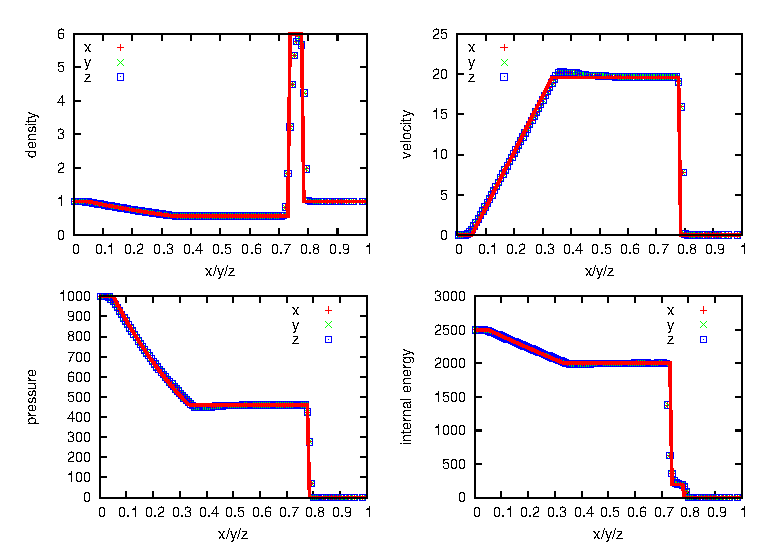
\includegraphics[width=5.0in]{test3_3d}
\caption{\label{fig:test3} \castro\ solution for the strong shock
  problem run in 3-d, along the $x$, $y$, and $z$ axes.  A coarse grid
  of 32 zones in the direction of propagation, with 2 levels of
  refinement was used.  The analytic solution appears as the red
  line.}
\end{figure}

Figure~\ref{fig:test3} shows the \castro\ output, run along all 3
coordinate axes in 3-d, compared to the analytic solution.  

The comparison to the analytic solution follows the same procedure as
described for the Sod's problem above.  The gnuplot script {\tt
  test3\_3d.gp} will generate the figure, from the 1-d slices created by
{\tt fextract} named {\tt test3x.out}, {\tt test3y.out}, and {\tt test3z.out}.


\subsection{Sedov Problem}

The \problem{Sedov} (or Sedov-Taylor) blast wave is a standard hydrodynamics
test problem.  A large amount of energy is placed into a very small
volume, driving a spherical (or cylindrical in 2-d Cartesian
coordinates) blast wave.  Analytic solutions were found by Sedov
\cite{sedov:1959}.  

A cylindrical blast wave (e.g.\ a point explosion in a 2-d plane) can
be modeled in 2-d Cartesian coordinates.  A spherical blast wave can
be modeled in 1-d spherical, 2-d axisymmetric (cylindrical $r$-$z$), or 3-d
Cartesian coordinates.  This provides a good test on the geometric
factors in the hydrodynamics solver.
We use a publically available code, {\tt sedov3.f}
\cite{timmes_sedov_code}, to generate the analytic solutions.

The \castro\ implementation of the Sedov problem is in {\tt Exec/hydro\_tests/Sedov}.
A number of different inputs/probin files are provided, corresponding
to different Sedov/\castro\ geometries.  The main ones are:

\begin{table*}[h]
\centering
{\small
\begin{tabular}{|l|l|p{2.25in}|} \hline
\multicolumn{1}{|c}{\em inputs file} &  \multicolumn{1}{|c}{\em probin file} & \multicolumn{1}{|c|}{\em description} \\
\hline
{\tt inputs.1d.sph} & {\tt probin.1d.sph} & Spherical Sedov explosion modeled in 1-d spherical coordinates \\[2mm]
%
{\tt inputs.2d.sph\_in\_cylcoords} & {\tt probin.2d.sph\_in\_cylcoords} & Spherical Sedov explosion modeled in 2-d cylindrical (axisymmetric) coordinates \\[2mm]
%
{\tt inputs.2d.cyl\_in\_cartcoords} & {\tt probin.2d.cyl\_in\_cartcoords} & Cylindrical Sedov explosion modeled in 2-d Cartesian coordinates \\[2mm]
%
{\tt inputs.3d.sph} & {\tt probin.3d.sph} & Spherical Sedov explosion modeled in 3-d Cartesian coordinates \\
\hline
\end{tabular}
\caption{\label{table:sedov_inputs} Sedov inputs files}
} % end small
\label{Table:Sod}
\end{table*}

In the Sedov problem, the explosion energy, $E_\mathrm{exp}$ (in units 
of energy, not energy/mass or energy/volume)
is to be deposited into a single point, in a medium of uniform ambient
density, $\rho_\mathrm{ambient}$, and pressure, $p_\mathrm{ambient}$.
Initializing the problem can be difficult because the small volume is
typically only a cell in extent.  This can lead to grid imprinting in
the solution.  A standard solution (see for example \cite{omang:2006}
and the references therein)
is to convert the explosion energy into a pressure contained within a
certain volume, $V_\mathrm{init}$, of radius $r_\mathrm{init}$ as
\begin{equation}
p_\mathrm{init} = \frac{(\gamma - 1) E_\mathrm{exp}}{V_\mathrm{init}} \enskip .
\end{equation}
This pressure is then deposited in all of the cells where $r <
r_\mathrm{init}$.  

To further minimize any grid effects, we do subsampling
in each zone: each zone is divided it into $N_\mathrm{sub}$ subzones in each
coordinate direction, each subzone is initialized independently, and
then the subzones are averaged together (using a volume weighting for
spherical or cylindrical/axisymmetric \castro\ grids) to determine the
initial state of the full zone.

For these runs, we use $\rho_\mathrm{ambient} = 1$,
$p_\mathrm{ambient} = 10^{-5}$, $E_\mathrm{exp} = 1$, $r_\mathrm{init}
 = 0.01$, and $N_\mathrm{sub} = 10$.  A base grid with 32 zones in each
coordinate direction plus 3 levels of refinement is used (the finest
mesh would coorespond to 256 zones in a coordinate direction).  The
domain runs from 0 to 1 in each coordinate direction.




Analysis routines for the Sedov problem are provided in
{\tt Castro/Diagnostics/Sedov/}.  These routines will
average the \castro\ solution over angles, using the proper geometric
weighting, to produce an average profile as a function of radius.
The following routines correspond to the inputs files described above:
\begin{table*}[h]
\centering
{\small
\begin{tabular}{|l|l|} \hline
\multicolumn{1}{|c}{\em inputs file} &  \multicolumn{1}{|c|}{\em analysis routine} \\
\hline
{\tt inputs.1d.sph} & {\tt fsedov1d.f90} \\
%
{\tt inputs.2d.sph\_in\_cylcoords} & {\tt fsedov2d\_sph\_in\_cylcoords.f90} \\
%
{\tt inputs.2d.cyl\_in\_cartcoords} & {\tt fsedov2d\_cyl\_in\_cartcoords.f90} \\
%
{\tt inputs.3d.sph} & {\tt fsedov3d\_sph.f90} \\
\hline
\end{tabular}
} % end small
\caption{\label{table:fsedov} Analysis routines for Sedov}
\end{table*}

\subsubsection{Spherical Blast Wave}

A spherical Sedov explosion can be modeled in 1-d spherical, 2-d
cylindrical (axisymmetric), or 3-d Cartesian coordinates, using the
inputs files described in Table~\ref{table:sedov_inputs}.  A 1-d radial
profile can be extracted using the appropriate {\tt fsedov} routine,
as listed in Table~\ref{table:fsedov}.  For example, to run and process
the 2-d cylindrical Sedov explosion, one would do:
\begin{enumerate}
\item in {\tt Exec/hydro\_tests/Sedov}, build the \castro\ executable in 2-d
\item run the spherical Sedov problem with \castro\ in 2-d cylindrical coordinates: \\
 {\tt ./Castro2d.Linux.Intel.Intel.ex inputs.2d.sph\_in\_cylcoords} 
\item build the {\tt fsedov2d\_sph\_in\_cylcoords} tool in 
{\tt Castro/Diagnostics/Sedov}.  
\item run {\tt fsedov2d\_sph\_in\_cylcoords} on the \castro\ output to generate 1-d radial
 profiles: \\
 {\tt fsedov2d\_sph\_in\_cylcoords.Linux.Intel.exe -s sedov\_2d\_sph\_in\_cyl.out $\mathtt{\backslash}$ } \\
 $~~~~~${\tt -p sedov\_2d\_sph\_in\_cyl\_plt00246} 
\end{enumerate}
A similar procedure can be used for the 1-d and 3-d spherical Sedov
explosions (with the output named {\tt sedov\_1d\_sph.out} and {\tt
  sedov\_3d\_sph.out} respectively).  Once this is done, the {\tt
  sedov\_sph.gp} gnuplot script can be used to make a plot comparing
the 3 solutions to the analytic solution, {\tt spherical\_sedov.dat}.

Figure~\ref{fig:sedov_sph} shows the comparison of the 3 \castro\
spherical Sedov explosion simulations to the analytic solution.

\begin{figure}[t]
\centering
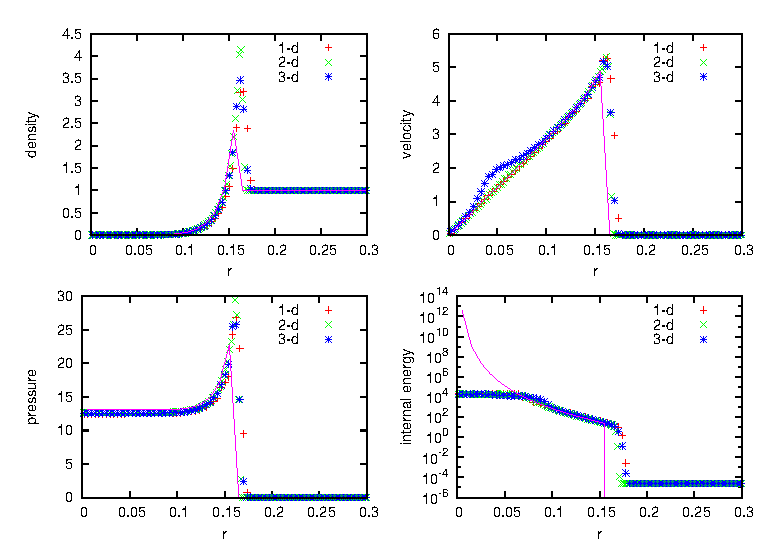
\includegraphics[width=5.0in]{sedov_sph}
\caption{\label{fig:sedov_sph} \castro\ solution for the Sedov blast wave problem
  run in 1-d spherical, 2-d axisymmetric, and 3-d Cartesian coordinates.
  Each of these geometries produces a spherical Sedov explosion.}
\end{figure}


\subsubsection{Cylindrical Blast Wave}

\begin{figure}[h]
\centering
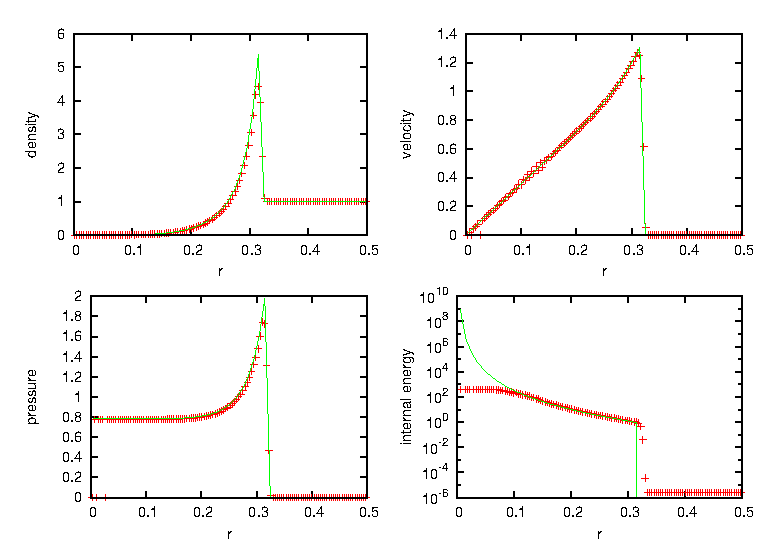
\includegraphics[width=5.0in]{sedov_cyl}
\caption{\label{fig:sedov_cyl} \castro\ solution for the Sedov blast wave problem
  run in 2-d Cartesian coordinates.  This corresponds to a cylindrical
  Sedov explosion.}
\end{figure}

\subsection{Rayleigh-Taylor}
2D.  Domain size 0.5 by 1.0.  256 by 512 cells, single level
calculation.  Periodic in x, solid walls on top and bottom in y.
Gamma law gas with $\gamma=1.4$, no reactions.  Zero initial velocity.
Constant $|\gb|=1$.  The density profile is essentially $\rho=1$ on
bottom, $\rho=2$ on top, but with a perturbation.  A single-mode
perturbation is constructed as:
\begin{equation}
\tilde y(x) = 0.5 + 0.01 \frac{\cos(4\pi x) + \cos(4\pi(L_x - x))}{2}
\end{equation}
We note that the symmetric form of the cosine is done to ensure that 
roundoff error does not introduce a left-right asymmetry in the problem.
Without this construction, the R-T instability will lose its symmetry
as it evolves.  This then applied to the interface with a tanh profile
to smooth the transition between the high and low density material:
\begin{equation}
\rho(x,y) = 1 + 0.5\left[1+\tanh\left(\frac{y-\tilde y(x)}{0.005}\right)\right]
\end{equation}
Hydrostatic pressure with $p=5.0$ at bottom of domain, assuming
$\rho=1$ on the lower half of the domain, and $\rho=2$ on the upper
half and no density perturbation.  We run to $t=2.5$ with piecewise
linear, old PPM, and new PPM.  CFL=0.9.  See Figure \ref{fig:RT}.
\begin{figure}[h]
\centering
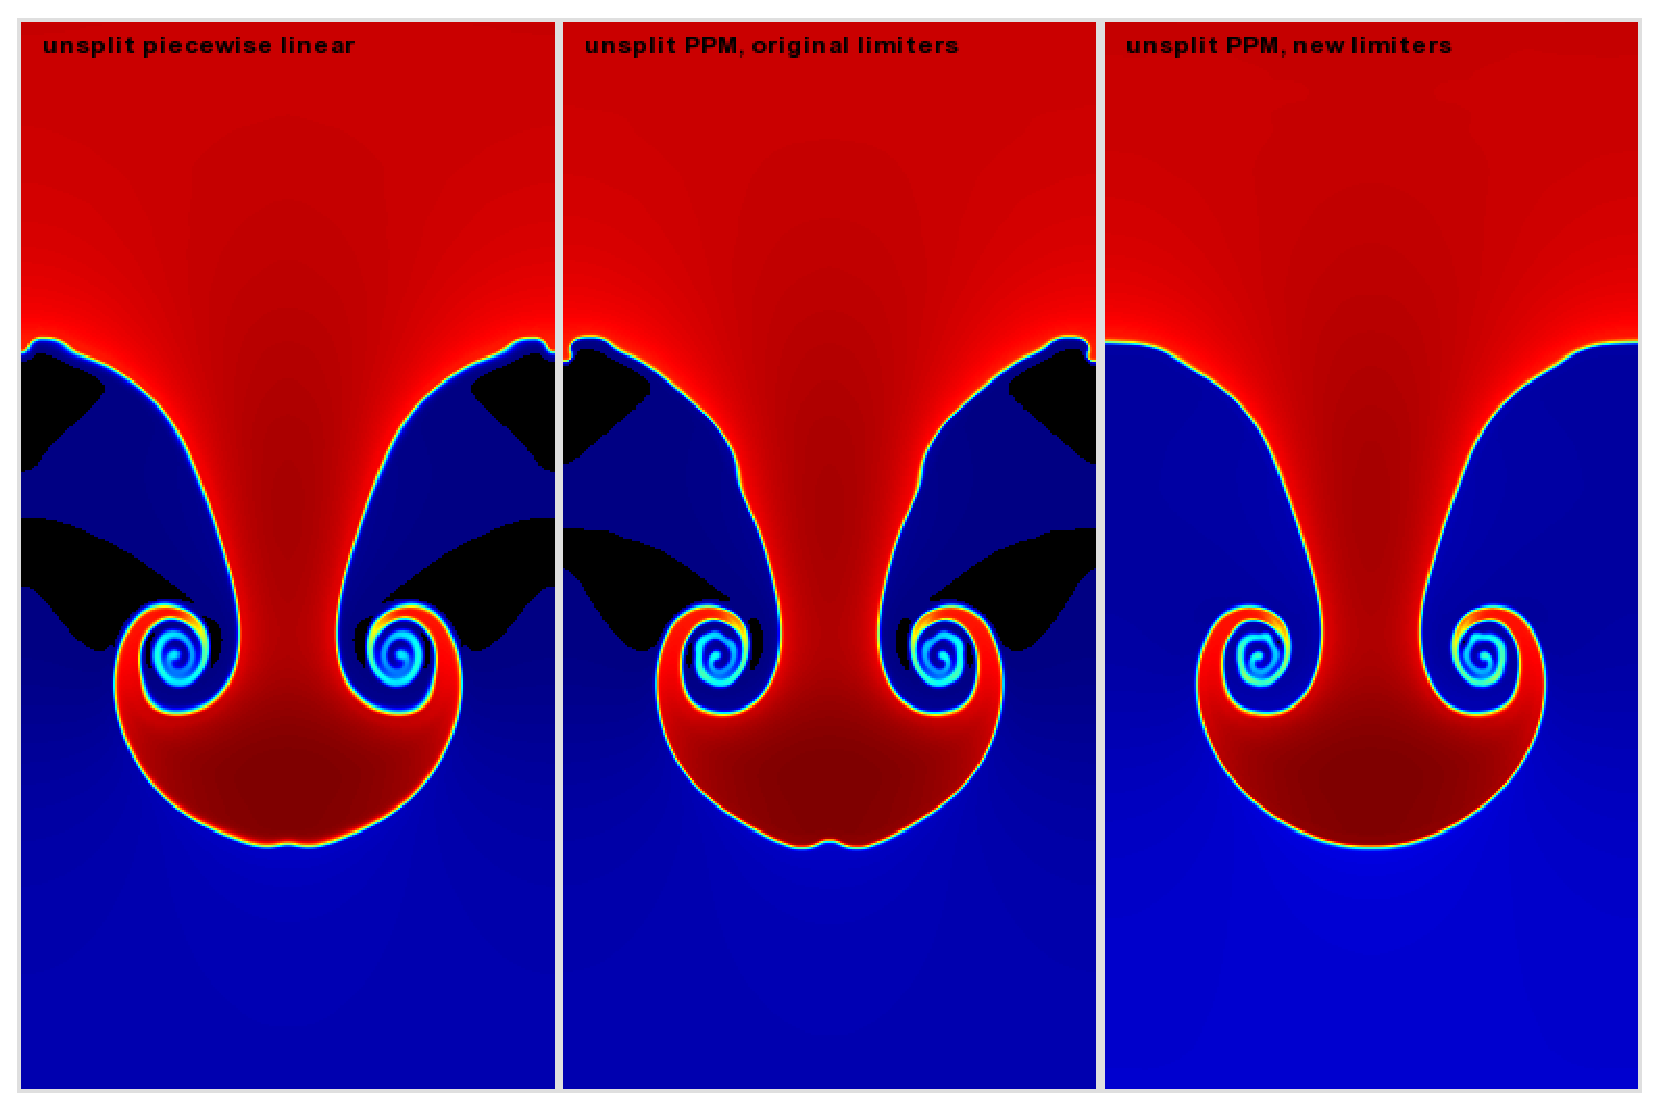
\includegraphics[width=6.5in]{RT_ppm_type}
\caption{\label{fig:RT}Rayleigh-Taylor with different PPM types.}
\end{figure}

%%%%%%%%%%%%%%%%%%%%%%%%%%%%%%%%%%%%%%%%%%%%%%%%%%%%%%%%%%%%%%%%%%%%%%%%%%%%%%%
\section{Gravity Test Problems}



%%%%%%%%%%%%%%%%%%%%%%%%%%%%%%%%%%%%%%%%%%%%%%%%%%%%%%%%%%%%%%%%%%%%%%%%%%%%%%%
\section{Radiation Test Problems}

There are two photon radiation solvers in \castro---a gray solver and a
multigroup solver.  The gray solver follows the algorithm outlined
in \cite{howellgreenough:2003}.  We use the notation described in that
paper.  In particular, the radiation energy equation takes the form
of:
\begin{equation}
\frac{\partial E_R}{\partial t} = 
 \nabla \cdot \left ( \frac{c \lambda(E_R)}{\kappa_R} \nabla E_R \right ) +
 \kappa_P (4 \sigma T^4 - c E_R )
\end{equation}
Here, $E_R$ is the radiation energy density, $\kappa_R$ is the
Roseland-mean opacity, $\kappa_P$ is the Planck-mean opaciy, and
$\lambda$ is a quantity $\le 1/3$ that is subjected to limiting to
keep the radiation field causal.  \castro\ allows for $\kappa_R$
and $\kappa_P$ to be set independently as power-laws.

\subsection{Light Front}

The light front problem tests the ability of the radiation solver to
operate in the free-streaming limit.  A radiation front is
estabilished by initializing one end of the computational domain with
a finite radiation field, and zero radiation field everywhere else.
The speed of propagation of the radiation front is keep in check by
the flux-limiters, to prevent it from exceeding $c$.


\subsection{Diffusion of a Gaussian Pulse}

The diffusion of a Gaussian pulse problem tests the diffusion term in
the radiation energy equation.  The radiation energy density is 
initialized at time $t = t_0$ to a Gaussian distribution:
\begin{equation}
E_R = (E_R)_0 \exp \left \{ - \frac{1}{4 D t_0} |r - r_0|^2 \right \} \enskip .
\end{equation}
As the radiation diffuses, the overall distribution will remain 
Gaussian, with the time-dependent solution of:
\begin{equation}
E_R = (E_R)_0 \frac{t_0}{t_0 + t} \exp \left \{ -\frac{1}{4 D (t_0 + t)} |r - r_0|^2 \right \}
\end{equation}


\subsection{Radiation Source Problem}

The radiation source problem tests the coupling between the radiation
field and the gas energy through the radiation source term.  The
problem begins with the radiation field and gas temperature out of
equilibrium.  If the gas is too cool, then the radiation field will
heat it.  If the gas is too hot, then it will radiate and cool.  In
each case, the gas energy and radiation field will evolve until
thermal equilibrium is achieved.

Our implementation of this problem follows that of
\cite{swestymyra:2009}.

\begin{figure}[h]
\centering
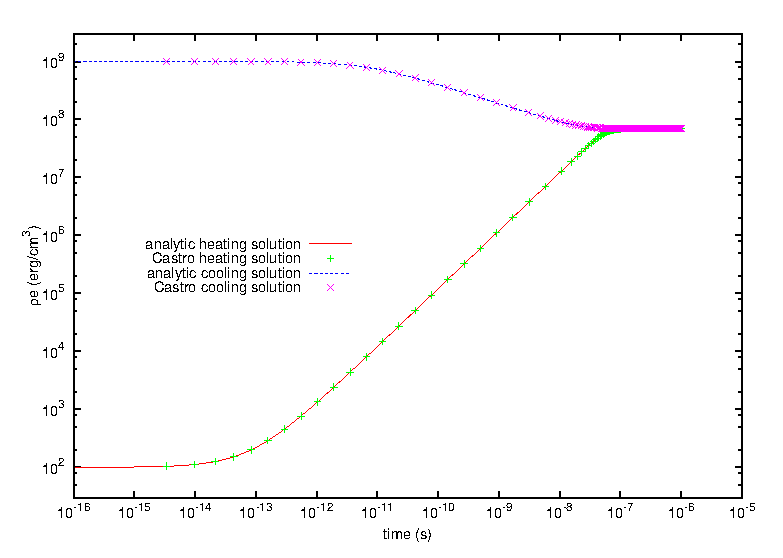
\includegraphics[width=5.0in]{radiating_source}
\caption{\label{fig:radsource} \castro\ solution for radiating source
  test problem.  Heating and cooling solutions are shown as a function
  of time, compared to the analytic solution.  The gray photon solver
  was used.}
\end{figure}


\subsection{Radiating Sphere}

The radiating sphere (\problem{RadSphere}) is a multigroup radiation
test problem.  A hot sphere is centered at the origin in a spherical
geometry.  The spectrum from this sphere follows a Planck
distribution.  The ambient medium is at a much lower temperature.  A
frequency-dependent opacity makes the domain optically thin for high
frequecies and optically thick for low frequency.  At long times, the
solution will be a combination of the blackbody radiation from the
ambient medium plus the radiation that propagated from the hot sphere.
An analytic solution exists \cite{graziani:2008} which gives the
radiation energy as a function of energy group at a specified time and
distance from the radiating sphere.

Our implementation of this problem is in {\tt Exec/radiation\_tests/RadSphere} and
follows that of \cite{swestymyra:2009}.  The routine that computes
the analytic solution is provided as {\tt analytic.f90}.

\begin{figure}[h]
\centering
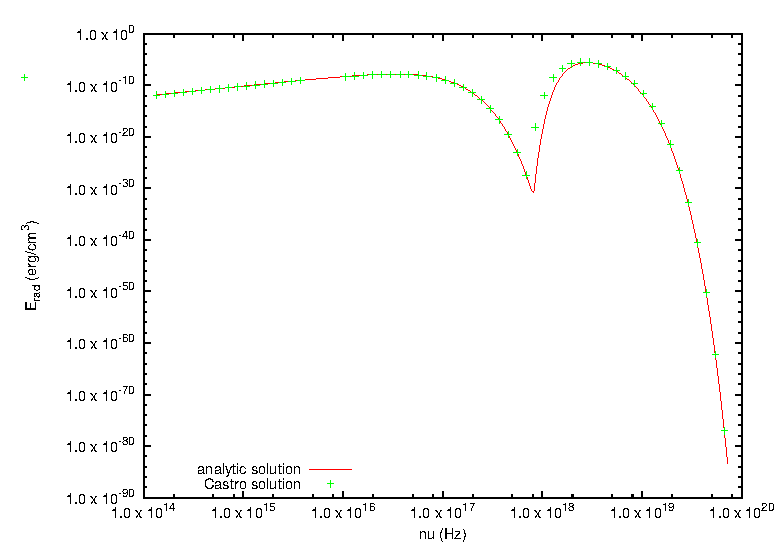
\includegraphics[width=5.0in]{radiating_sphere}
\caption{\label{fig:radsphere} \castro\ solution for radiating sphere problem,
  showing the radiation energy density as a function of energy group.
  This test was run with 64 photon energy groups.}
\end{figure}


\section{Regression Testing}

An automated regression test suite for \castro\ (or any \boxlib-based
code) written in Python exists in {\tt BoxLib/Tools/RegressionTesting}.
Details of its use are provided in the \boxlib\ User's Guide.
